% E9 pipeline diagram v2 — the two cleaning orders, boxes bound to Farid (2014) algorithms
% Compile: pdflatex e9-pipeline.tex
% Design: Okabe-Ito colorblind-safe palette; labels carry all meaning (no color-only encoding).
\documentclass[border=8pt]{standalone}
\usepackage{tikz}
\usetikzlibrary{positioning, arrows.meta, decorations.pathreplacing}

\definecolor{okblue}{HTML}{0072B2}
\definecolor{okorange}{HTML}{E69F00}
\definecolor{okgreen}{HTML}{009E73}
\definecolor{okpurple}{HTML}{CC79A7}

\begin{document}
\hyphenpenalty=10000
\exhyphenpenalty=10000
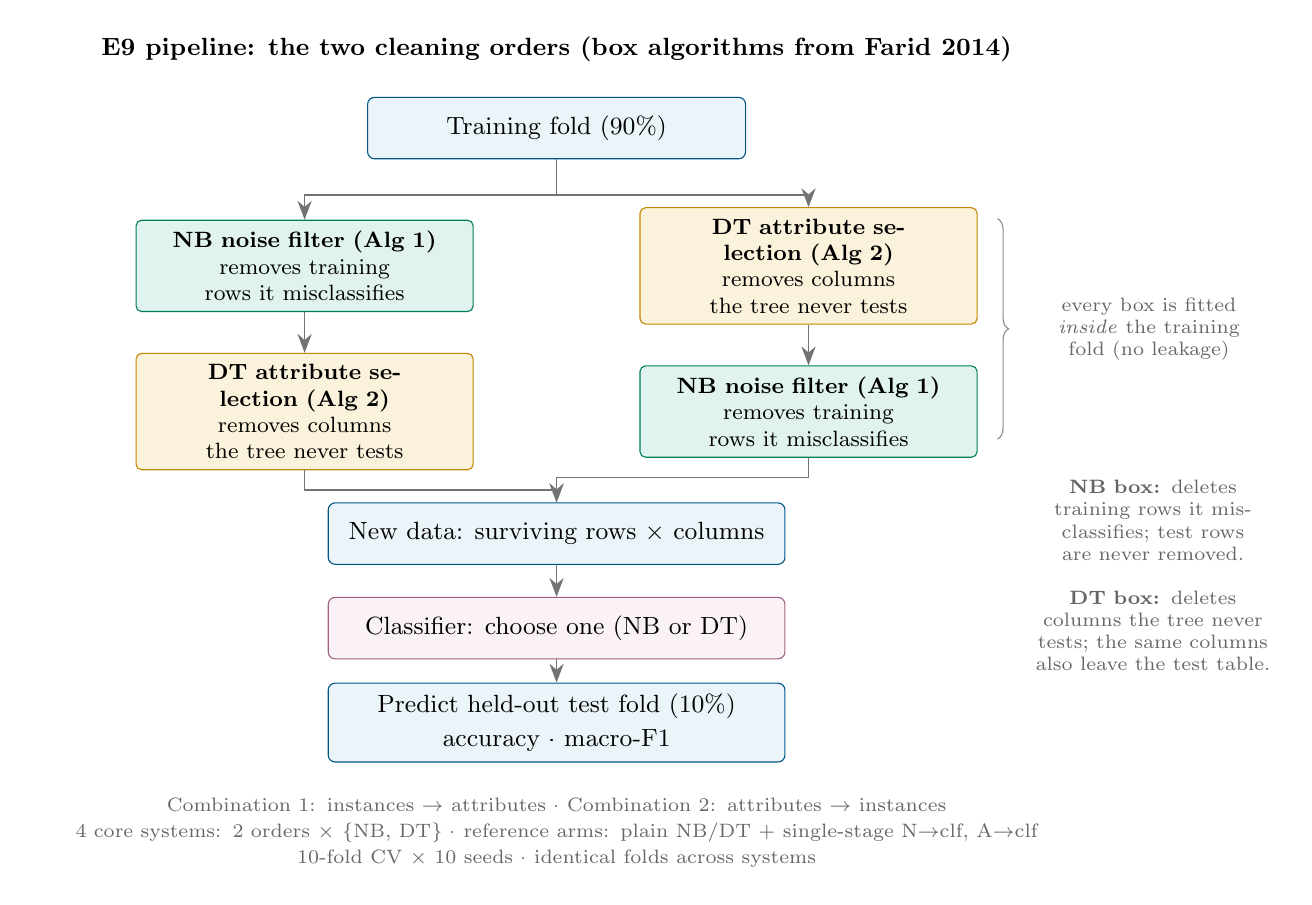
\begin{tikzpicture}[
  font=\small,
  every node/.style={align=center},
  flow/.style={-{Stealth[length=2.4mm,width=1.8mm]}, draw=black!55, line width=0.6pt},
  data/.style={draw=okblue!75!black, fill=okblue!8, rounded corners=2.5pt,
               inner sep=4pt, minimum height=0.78cm, minimum width=4.8cm},
  chipN/.style={draw=okgreen!80!black, fill=okgreen!12, rounded corners=2pt,
                inner sep=4pt, text width=4.0cm, font=\footnotesize},
  chipA/.style={draw=okorange!85!black, fill=okorange!14, rounded corners=2pt,
                inner sep=4pt, text width=4.0cm, font=\footnotesize},
  clf/.style={draw=okpurple!80!black, fill=okpurple!10, rounded corners=2.5pt,
              inner sep=4pt, minimum height=0.78cm, minimum width=5.8cm},
  note/.style={font=\scriptsize, text=black!60},
]

% ---------- title ----------
\node[font=\small\bfseries] (title) at (0,1.0)
  {E9 pipeline: the two cleaning orders (box algorithms from Farid 2014)};

% ---------- input ----------
\node[data] (train) at (0,0) {Training fold (90\%)};

% ---------- lane 1: instances first, then attributes ----------
\node[chipN] (n1) at (-3.2,-1.75)
  {\textbf{NB noise filter (Alg 1)}\\removes training rows it misclassifies};
\node[chipA] (a1) at (-3.2,-3.60)
  {\textbf{DT attribute selection (Alg 2)}\\removes columns the tree never tests};

% ---------- lane 2: attributes first, then instances ----------
\node[chipA] (a2) at (3.2,-1.75)
  {\textbf{DT attribute selection (Alg 2)}\\removes columns the tree never tests};
\node[chipN] (n2) at (3.2,-3.60)
  {\textbf{NB noise filter (Alg 1)}\\removes training rows it misclassifies};

% ---------- merge ----------
\node[data, minimum width=5.8cm] (newdata) at (0,-5.15) {New data: surviving rows $\times$ columns};
\node[clf] (clf) at (0,-6.35) {Classifier: choose one (NB or DT)};
\node[data, minimum width=5.8cm] (result) at (0,-7.55)
  {Predict held-out test fold (10\%)\\[1pt] accuracy \textperiodcentered{} macro-F1};

% ---------- arrows ----------
\draw[flow] (train.south) -- ++(0,-0.45) -| (n1.north);
\draw[flow] (train.south) -- ++(0,-0.45) -| (a2.north);
\draw[flow] (n1.south) -- (a1.north);
\draw[flow] (a2.south) -- (n2.north);
\draw[flow] (a1.south) -- ++(0,-0.25) -| (newdata.north);
\draw[flow] (n2.south) -- ++(0,-0.25) -| (newdata.north);
\draw[flow] (newdata.south) -- (clf.north);
\draw[flow] (clf.south) -- (result.north);

% ---------- right annotations ----------
\draw[decorate, decoration={brace, amplitude=4pt}, draw=black!45]
  (5.6,-1.15) -- (5.6,-3.95);
\node[note, anchor=west, text width=3.0cm] at (5.9,-2.55)
  {every box is fitted \emph{inside} the training fold (no leakage)};
\node[note, anchor=north west, text width=3.1cm] at (5.9,-4.35)
  {\textbf{NB box:} deletes training rows it misclassifies; test rows are never removed.};
\node[note, anchor=north west, text width=3.1cm] at (5.9,-5.75)
  {\textbf{DT box:} deletes columns the tree never tests; the same columns also leave the test table.};

% ---------- footer ----------
\node[note, text width=13.2cm] at (0,-8.95)
  {Combination 1: instances $\rightarrow$ attributes \textperiodcentered{}
   Combination 2: attributes $\rightarrow$ instances\\[1.5pt]
   4 core systems: 2 orders $\times$ \{NB, DT\} \textperiodcentered{}
   reference arms: plain NB/DT $+$ single-stage N$\rightarrow$clf, A$\rightarrow$clf\\[1.5pt]
   10-fold CV $\times$ 10 seeds \textperiodcentered{} identical folds across systems};

\end{tikzpicture}
\end{document}
